\section{Esoterica - a lead close to camp X-Ray}
\begin{marginfigure}
\begin{tikzpicture}
\node [name-dest] (box){%
    \begin{minipage}{0.80\textwidth}
     \begin{itemize}
    \item William French
    \item James O'Hanlon
    \end{itemize}
    \end{minipage}

};
\node[fancytitle, right=10pt] at (box.north west) {Your Mum};
\end{tikzpicture}
\end{marginfigure}

James wanted me to take him camping, and after talking to a lot of people about easy leads (I didn't really know what I was doing), it looked like \passage{Esoterica} off \passage{Prince Consort Road} was the safest bet. It took a bit of detective work to find it. Dave W had suggested finding the PSS Esoterica had been tied into, and then looking around that area. Around that PSS the first possibility was a strange multilevel streamway which I had vague memories (fantasies?) of being told by a different James in 2010 was the source of the name '\passage{Esoterica}' because it looked weird. That didn't go anywhere, and we had a closer look at the PSS and it turned out there was a map on the other side that was obscured by a layer of mud. We washed away this mud with water and after a bit of squinting concluded that the treasures we were seeking were down a crawl further back in \passage{Prince Consort Road}. 

This led to a dry climb down, and then a small wet rift. There was a dry side passage, but we didn't go into it and instead forced our way through the streamway until we got to a couple of rigged pitches that indicated we had found what we were looking for, and soon reached the limit of exploration which was a 5m undescended pitch. I tried to teach James how to bolt, but as it was in a rather awkward position gave up and slowly put in 3 bolts while James froze. At the bottom of that pitch was another pitch, but as we had achieved the original goal of pushing something we decided to not bother. We called it '\passage{Your Mum}' because that's a very witty name. 

On the way out, one of the naturals that had been rigged (by unnamed other people) on \passage{Esoterica} failed on James. I heard him shouting something unintelligible as he went up the pitch, and when it was my turn found that the deviation wasn't keeping me out of the water any more, and this was because a chockstone the rope was tied to had fallen into the rift. At least the other natural that was used on the pitch held firm and kept us both alive.


When I went caving with Tanguy for my last trip of the expedition, I took him to a dry way on in Esoterica that me and James had encountered a few days but did not look closely at. After my first trip to that part of the cave, Jarv had mentioned a pitch that he and Oli had half bolted a few years ago, and left a note after a driver broke. This made no sense at the time, but when Tanguy and I explored the dry side passage, it soon led to the wet pitch Jarv had been describing. Also, if you ignored the pitch and kept going straight, it broke out into a second connection to \passage{Prince Consort Road}. This tangle of passages may partly explain why people seemed to have been so confused talking about \passage{Esoterica} in the past. 

After finishing the bolting 2 years later we descended a 15m pitch to find that the streamway continued, but very quickly led to a pitch head that was too narrow to descend. We took it in turns hammering away at this with a moderate amount of success. I spent a while slowly wedging myself further and further into the crack until Tanguy gently suggested we called it a day, and leave it for someone with a chisel to break through. Since Tanguy is French, we gave the passage a French name, and so the name \passage{Serrure} (keyhole) was chosen. We had a fair amount of time to kill before we could go back to camp, so we took the time to survey the loop we had found in  \passage{Esoterica}/ \passage{Prince Consort Road}.
\name{William French}

\begin{marginfigure}
\centering
\frame{\includegraphics[width= \linewidth]{"images/2014/esoterica-2014/will-at-camp".jpg}}
\label{Will at camp}
\caption{William French kits up at camp X-Ray before going to explore the \passage{Esoterica} stream passage --- Jarvist Frost}
\end{marginfigure}

On the one hand, Rhys and Jarv had gone to investigate the deep leads and were intent on making the most of their trip. William and I on the other hand had settled for a more pleasant and laid back pushing trip close to camp on the 'connection branch' at the bottom of \passage{Cheetah}. We were to drop a pitch Jarv and Oli had the misfortune of finding, being unable to descent it as their only spitz driver broke during the bolting process. We booked two nights at camp \passage{X-Ray} and the plan was to follow the then sleep-push-sleep-get out routine. Our eagerness to go underground was enhanced by the incoming mass of black cumulonimbi on \passage{Migovec}, but the journey down was rather uneventful.

\begin{marginfigure}
\begin{tikzpicture}
\node [name-dest] (box){%
    \begin{minipage}{0.80\textwidth}
     \begin{itemize}
    \item William French
    \item Tanguy Racine
    \end{itemize}
    \end{minipage}

};
\node[fancytitle, right=10pt] at (box.north west) {Serrure};
\end{tikzpicture}
\end{marginfigure}

Upon leaving \passage{X-Ray} on the morning, we heard the roar of \passage{Zimmer}. We also heard tales of Rhys and Jarv who'd turned back because of flood conditions. I still remember awakening to the scraping of PVC against rock and marvelling at  the sight of their dripping, glistening, black tacklesacks. William and I successively went to look at the mighty \passage{Zimmer} pitch. Our floodlights inundated the space, and so did a torrential rain. One after the other, we raced across the boulders strewn on the floor, jammers at the ready, and ascended into the deep gouge that led to \passage{Cheetah} with lightning speed.

Miserable and wet, we descended the muddy pitch and followed \passage{Prince Consort Road}, traversed over a small pitch, and carried on the passage for a little while until the \passage{Esoterica} lead was spotted. We quickly found the two year old notes as well as one of the bolts in the wall. A cascade could be seen down the pitch, and its development was near vertical widening towards the bottom. This meant a straight hang to the bottom was possible. I rigged a Y-hang after putting two bolts, using one of the existing bolts as back up. The hang dropped nicely to the bottom of the pitch. I quickly abseiled down, with complete disregard to the normal approach: a gradual abseil helps one spot possible windows on the way down! 

\begin{figure}[t]
	\checkoddpage \ifoddpage \forcerectofloat \else \forceversofloat \fi
    		\centering
		\frame{\includegraphics[width=\linewidth]{"images/2014/esoterica-2014/plan_serrure".png}} 
    
   		\caption{A plan of the passages branching of \emph{Prince Consort Road}, in particular a small, disconcerting loop surveyed by Tanguy Racine and William French. The lead in \emph{Serrure} is ongoing at the time of writing
    		 --- scanned from 2014 underground logbook}
		 \label{serrure scan}
\end{figure}

Instead I found myself at the bottom, with a bit of spray coming off the walls into my face. I could hardly look up without closing one eye. Slowly William's light came down, with him in tow. From where we stood, a drier alcove with pristine mud formations could be reached by a small down climb. The stream disappeared in the rift below. By shining our light down, it was almost possible to make out a continuation, but the rift looked formidably tight. The only place where it widened was obviously where the water carved a notch before cascading down. Below there was space enough to use safe SRT, the only barrier was the very tight pitch head at the top.

Slightly further downstream of the rift, there seemed to be the possibility of dislodging a few notches in the wall to make it passable, but since we only had one hammer, we resolved to put two spitz in the rock first, try the squeeze, and if needed enlarge it. I went up to grab the rest of the rope while William put the bolts. After a while, both were in, we tied in our rope and tried our luck. But unfortunately, the passage was as tight as a letterbox and we failed to make any progress. With a sigh of disappointment, we packed up our gear, coiled the now muddy rope and put it back in the tackle sack before starting our survey. The keyhole passage which the water had carved became the '\passage{Serrure}'.
\name{Tanguy Racine}

\begin{figure*}[b!]
\centering
\frame{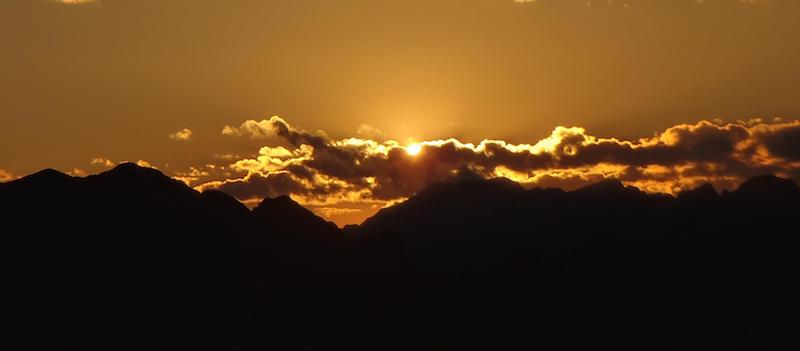
\includegraphics[width=\textwidth]{images/2014/esoterica-2014/izi-sunset.jpg}}
\caption{Sunset over the Krn mountain ranges --- Iztok Mozir}
\label{SS2014}
\end{figure*}